We've presented different dynamical models for the central region of J1331. Some of them capture the observed kinematics, but none of them work at both small and large radii. In the following we discuss possible reasons, also by comparing our results to previous work.

\subsection{On J1331's central stellar mass-to-light ratio} \label{sec:MLdiscussion}

Some of the ambiguities in recovering J1331's matter distribution could be resolved by learning more about stellar populations with different IMFs in J1331. In particular, a sophisticated guess for the stellar mass-to-light ratio in the bulge could be compared to our very reliable measurement of the total mass-to-light ratio inside the Einstein radius (see Table \ref{tab:einsteinML}). This would then either support or contradict the presence of a significant amount of DM in the bulge.

Traditional choices for the IMF are the bottom-heavy IMF by \citet{Salpeter1955},
$$\xi(m) \propto m^{-x}, x=2.35,$$
where $\xi(m) \diff m$ is the number of stars with mass $m$ in $[m,m+\diff m]$, and the IMFs by \citet{2002Sci...295...82K} and \citet{Chabrier2003}, which are in agreement with each other and predict less low-mass stars.

\citet{Ferreras} found a relation between the central stellar velocity dispersion $\sigma_0$ in early-type galaxies and the IMF slope $x$; a higher $\sigma_0$ suggests a more bottom-heavy IMF. For a unimodal (Salpeter-like) IMF and $\sigma_0 \simeq 200~\text{km s}^{-1}$ in J1331 (see Figure \ref{fig:kinematics}) they predict $x \approx 2.33$, which is close to the standard Salpeter slope, also supported by \citet{2014MNRAS.438.1483S}. When assuming a bi-modal (Kroupa-equivalent-like) IMF, \citet{Ferreras} predict $x \approx 2.85$ for J1331's central velocity dispersion. This is more bottom-heavy than the standard \citet{2002Sci...295...82K} IMF. Overall, the central velocity dispersion suggests a rather bottom-heavy IMF in J1331's bulge and therefore large stellar mass-to-light ratio. 

\citet{SWELLSI} estimated J1331's stellar bulge mass given a Salpeter IMF and measured the I-band AB magnitude of the bulge. Transformed to a stellar I-band mass-to-light ratio, their results would correspond to $\Upsilon_\text{I,*}^\text{sal} = 4.7 \pm 1.2$ (see Table \ref{tab:previousresults}). This is not too far from $\Upsilon_\text{I,*} = 4.2 \pm 0.2$ (see Table \Wilma{[TO DO]}), which we found when including a NFW halo in the JAM modelling.

When \citet{SWELLSI} assumed a Chabrier IMF, their result translates to $\Upsilon_\text{I,*}^\text{chab} = 2.5 \pm 0.6$ (see Table \ref{tab:previousresults}). In Section \ref{sec:results_JAM_SB} we created a dynamical model from only the surface brightness distribution and an increasing mass-to-light ratio profile without additional DM halo. We found that such a model would be perfectly consistent with the Einstein mass, predict a total $\Upsilon_\text{I,tot}(R'\sim0) = 2.53$---being consistent with the Chabrier IMF estimate by \citet{SWELLSI}---and rise quickly to $\Upsilon_\text{I,tot}(R'\gtrsim R_\text{ein}) \gtrsim 6$.

We also compare our results from Section \ref{sec:results_JAM_NFW} with the study by \citet{SWELLSV}. They found that the bulge of J1331 has an IMF \emph{more} bottom-heavy than the Salpeter IMF from fitting a NFW halo to (1) the Einstein mass and (2) gas kinematics at larger radii $\gtrsim 8''$. In Section we fitted a mass model with NFW halo to (1) the Einstein mass and (2) stellar kinematics within $\sim 3.5''$. Our best fit $\Upsilon_\text{I,*} = 4.2 \pm 0.2$ (see Table \ref{tab:modelB4_bestfit}) indicates a \emph{less} bottom-heavy IMF than the Salpeter IMF. \cite{SWELLSV} found systematically lower NFW halo masses ($v_\text{circ,halo}(5'') \sim 120~\text{km s}^{-1}$ according to their Figure 2) than we did ($v_\text{circ,halo}(5'') \sim 200~\text{km s}^{-1}$).


%==============
\begin{table*}
\centering
\begin{tabular}{cccccc}
\hline\hline
& & \multicolumn{2}{c}{Chabrier IMF} & \multicolumn{2}{c}{Salpeter IMF}\\
      &  $L$ [$10^{10}L_{\odot}$]                & $M_*$ [$10^{10}M_\odot$]               & $\Upsilon_\text{I,*}^\text{chab}$ & $M_*$ [$10^{10}M_\odot$] & $\Upsilon_\text{I,*}^\text{sal}$ \\\hline
bulge &   $3.10 \pm 0.15 $  & $7.8 \pm 1.8$ & $2.5 \pm 0.6$ & $14.5 \pm 3.7 $ & $4.7 \pm 1.2$ \\
disk  &   $2.35 \pm 0.11 $  & $2.9 \pm 0.7$ & $1.2 \pm 0.3$ & $5.2 \pm 1.1$ & $2.2 \pm 0.5$ \\
total &   $5.45 \pm 0.19$ & $10.6 \pm 1.9$& & $19.7 \pm 3.9$&\\\hline
\end{tabular}
\caption{Total I-band luminosity, stellar mass and mass-to-light ratio, calculated from the I-band AB magnitudes and stellar masses found for J133's bulge and disk by \citet{SWELLSI} (their table 2) for comparison with this work. The transformation from AB magnitudes to the Johnson-Cousins I-Band used the relation $I[\text{mag}] = I[\text{ABmag}] - 0.309$ from \citet{FG1994} (their table 2). For the conversion from apparent magnitude to total luminosity the redshift $z=0.113$ \citet{SWELLSIII} was turned into a luminosity distance using the cosmology by \citet{WMAP5cosm}. }
\label{tab:previousresults}
\end{table*}
%==============

\subsection{On J1331's central kinematics}

%==============
\begin{figure}
\centering
  \includegraphics[width=0.9\linewidth]{fig/B4_jam_profiles_errors_short_vcirc.ps}
  \caption{Circular velocity curve. \Wilma{[TO DO: Write caption]}}
  \label{fig:vcirc_comparison}
\end{figure}
%==============

In Figure \ref{fig:vcirc_comparison} we compare the circular velocity curve found by \citet{SWELLSV} with a mass-follows-light model scaled to fit our Einstein mass (by multiplying the light distribution in Table \Wilma{[TO DO]} with $\Upsilon_\text{I,tot}^\text{ein} = 5.6$). Within $R < 5''$ they agree with each other. 

The models in this work used more than just the Einstein mass to constrain the matter distribution at small radii: The lens mass model constrained also the shape of the mass distribution within the lensing image configuration at $R_\text{ein} \sim 1''$. The dynamical models used stellar kinematics inside $R' \simeq 3.5''$ \Wilma{[TO DO: Check]}. We compare the lens mass model's $v_\text{circ}$ (for $\alpha=1.0\pm 0.1$) with the NFW JAM model (Table \Wilma{[TO DO]}) in Figure \ref{fig:vcirc_comparison} as well. Within and around $R_\text{ein}$ they are consistent with each other, even though they where independently derived. They do not agree with the result by \citet{SWELLSV} and in Section \ref{sec:results_JAM_SB} we showed, that ``mass-follows-light'' is not a good model for J1331.

Overall, we were not able to find a consistent explanation for J1331's central $v_\text{rms}$ dip. It cannot be due to tangential velocity anisotropy in the center alone (see Section \ref{sec:results_JAM_SB}, Figure \ref{fig:JAM_modelA2}). It also cannot be explained by a strong contribution of DM inside the bulge together with a moderate tagential velocity anisotropy, because the corresponding DM halos would still be too massive to fit the data in the outer regions (see Section \ref{sec:results_JAM_NFW}, Figure \ref{fig:modelB4_vrms}]).

Another feature in the stellar kinematics, that none of our JAM models was able to reproduce in the slightest and which we therefore excluded in the modelling, was the dip in $v_\text{rms}$ around $\sim 6''$, which occurs around the transition from bulge to disk (see Figures \ref{fig:F814W} and \ref{fig:kinematics}).

\subsection{On J1331's possible merger history}

\Wilma{[TO DO: Remove minor in merger.]}

J1331 has a large counter-rotating stellar core within $\sim 2''$. This suggests a process in J1331's past in which two components with angular momenta oriented in opposite directions were involved. Accretion of gas on retrograde orbits and subsequent star formation could lead to a younger and counter-rotating stellar population \Wilma{[TO DO: REF]}. However, to form enough stars such that the net rotation of the large and massive core is retrograde, a very large amount of gas would have had to be accreted by J1331---which is not very likely [TO DO: REF]. 

Another scenario are galaxy mergers. Major mergers including large amounts of gas can form kinematically decoupled cores (KDCs), see e.g., \Wilma{[TO DO: REF: Lauren Hofman et al 2010 - read paper how this fits with the reverse color gradient]}. During a minor merger, the dense nucleus of a satellite galaxy on a retrograde orbit could survive the dissipationless accretion and could spiral to the core due to tidal friction \citep{1984ApJ...287..577K}. Usually large bulges of spirals or ellipticals are reddest in the center and become bluer further out.  Because star formation in low-mass satellite galaxies occurred later than in massive galaxies \Wilma{[TO DO: REF]}, the merger remnant would now host a younger and bluer population with lower velocity dispersion within the older and redder bulge of the massive progenitor. Such a reverse color gradient could correspond to an increasing stellar mass-to-light ratio.

The merger theory could explain and support our findings from dynamical modelling and the previous sections, that J1331 might have an increasing stellar mass-to-light ratio within its core. 

\subsection{On possible modelling failures and speculations how to resolve them}

\Wilma{[TO DO: Include in discussion: Kinematic twist due to merger. Bulge and disk have different kinematic major axis, and the measured velocities in the disk, which are off from the major axis, are much lower than the actual maximum vcirc. Could explain the dips in the outer regions.]}

Another effect that minor mergers can have on galaxies are a misalignement (warp) of the photometric and kinematic major axis \Wilma{[TO DO: REF]}. Would this be the case for J1331 the assumption of axisymmetry is not true anymore and our dynamical modelling would fail.

Mergers also could have changed the 3D shape of the dark matter halo and the NFW halo was therefore not a good model for J1331's dark matter halo. We also tried to model J1331 with a cored logarithmic halo. However, due to degeneracies in the modelling, we were not able to either constrain the profile for a cored logarithmic halo, or to rule it out. 

\Wilma{[TO DO: Include in this discussion the findings from the color profile.]}

This could indicate that there might be a less bottom-heavy, more bluish population, with an IMF close to the Chabrier IMF, in the very center of J1331.

\subsection{Future work}

Standard JAM modelling approaches seem not to work for J1331. A JAM model for J1331 would need to allow for stellar mass-to-light ratio gradients within the galaxy, velocity anisotropy and a dark matter halo. Because of degeneracies between stellar and dark mass, and matter distribution and anisotropy profile, such a dynamical model would not lead to very tight constraints on the model parameters.  A search for colour gradients in J1331 and/or investigation of absorption line indices could support or contradict the suspicion of the existence of stellar mass-to-light ratio gradients in J1331. Subsequently detailed stellar population analyses of the spectra taken along J1331's major axis should be conducted to constrain the mass-to-light ratio reliably.  \Wilma{[TO DO: Include in this discussion the findings from the color profile.]}

In addition, the dynamical modelling should use more of the available information on J1331 and fit dynamics (stellar and gas kinematics from \citet{SWELLSV}) simultaneously with the gravitational lensing (image positions, shape and even flux ratios) in a similar fashion to \citet{SWELLSIV}. To also model the extent, shape and flux of the lensing images, the method by \citet{2004ApJ...611..739T,2003ApJ...590..673W} could be employed, which models the surface brightness distribution of the images and source on a pixelated grid. However, for this to work a good model for the galactic extinction would be needed. 

High-resolution integral-field spectroscopy could help with this, allow for spatially resolved stellar population analysis and dynamical modelling in two dimensions. \Wilma{[TO DO: Include in this discussion that this could also help test, if the vrms dip is maybe because of twist, i.e., the measurements where not done along the major axis in the disk]} This would lead to much better understanding of J1331's structure and mass distribution and therefore answer questions on how minor mergers might modify spiral galaxies.

\Wilma{[TO DO: Include in discussion: High resolution IFU: high spatial resolution --> to resolve small features. High spectral resolution --> because the velocity dispersion in the outer regions of the galaxy are very low and to measure them accurately, need high spectral resolution.]}



\Wilma{[TO DO: Include the following discssion somwhere: The above discussion motivates the following speculation: In the absence of a strong DM contribution in the center, the overall stellar-mass-to-light ratio within the Einstein radius indicates a bottom-heavy IMF close to the Salpeter IMF, consistent with estimates from the velocity dispersion. At the same time the central dip can then be only explained, if there was an increase in stellar mass-to-light ratio with radius \textit{within} the bulge. \emph{If} there was a central stellar population with an IMF close to the \citet{Chabrier2003} IMF, surrounded by a more bottom-heavy population, the central stellar kinematics would be well explained and be fully consistent with the lensing results. (According to Figure \ref{fig:lenscompareboth} the lensing result might not predict a mass to light ratio gradient inside $R_\text{ein}$, but then again the mass slope $alpha=1$ was only weakly constrained.) The disk of J1331 has a lower $\Upsilon_\text{I,*}$ than the bulge (see Table \ref{tab:previousresults} according to \citet{SWELLSI}). Such a drop in $\Upsilon_\text{I,*}$ at the transition region from bulge to disk around $\sim 5''$ could lead to the observed drop in $v_\text{rms}$, while an increasing contribution of a lower mass DM halo at larger radii as found by \citet{SWELLSV}, would recover the kinematics in the out regions of J1331's disk.]}

\Wilma{[TO DO: Why are disk and bulge mass in SWELLS I different to the one in SWELLS IV??]}

